\label{chapter:Avaliacao}

\par
\textcolor{red}{Nesta seção será apresentado os processos e avaliações dos testes do projeto, com intuito de expor se os modelos de classificação e associação foram bem sucedidos, se a taxa de precisão da classificação alcançou a porcentagem do que se era esperado, se foi gerado as regras que eram necessarias para a avaliação dos dois modelos e entre outros.}

\par
\textcolor{red}{Para a avaliação do experimento, no processo de mineração, foi utilizado um notebook pessoal da marca DELL do modelo Inspiron 5558, que possui um processador Intel(R) Core(TM) i5-5200U CPU @ 2.20 GHz com uma mémoria instalada de 16 GB. Para o uso dos algoritmos de classificação e associação para mineração e avaliação, foi utilizado a versão estável 3.8.3 do software WEKA.}

\section{Avaliando com o algoritmo J48}

\par
\textcolor{red}{De forma para validar o modelo feito pela atividade de classificação, foi utilizada um filtro do Explore do WEKA chamado de \textit{RemovePercentage} para poder fazer a separação da base de dados para treinamento e teste. Possuindo 1.574 registros, a base de dados foi separada em duas partes, tendo como 70\% dos dados para treinamento com 1086 instancias e 30\% dos dados para teste com 486 instancias. Após o processo de utilizar o modelo de classificação do conjunto de treinamento para testar no conjunto de teste, o algoritmo J48 obteve como resultado uma precisão de 57\% das instâncias classificadas corretamente e de aproximadamente 43\% das instancias classificada incorretamente, como demonstrado na Figura XX.}

\par
\begin{figure}[!htp]
	\begin{center}
    \caption{\label{fig:waveform_fig} Resultado de acurácia do modelo de validação.}
	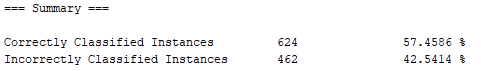
\includegraphics[scale=0.99]{Figuras/Modelo_de_validacao.png}
	\end{center}
    \legend{Fonte: Próprio autor.}
\end{figure}

\par
\textcolor{red}{Na base de dados balanceada, através do software WEKA, á análise por arvore de decisão foi feita utilizando o algoritmo J48, usando a opção \textit{cross-validation} para a sua execução, com um valor para fold igual a dez e com a variável dependente Aprovado. A árvore de decisão foi capaz de identificar corretamente aproximadamente 53\% instâncias das 1.574 inseridas, como apresentado na Figura XX. Pode se notar que a taxa de acurácia obtida pelo algoritmo tem um valor aproximado da taxa do modelo de validação que foi mencionado, comprovando dessa forma que o modelo avaliado é considerado útil para ser utilizado.}

\par
\begin{figure}[!htp]
	\begin{center}
    \caption{\label{fig:waveform_fig} Resultado de acurácia do modelo de base de dados.}
	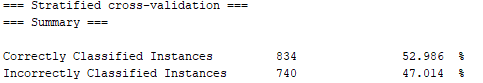
\includegraphics[scale=0.99]{Figuras/Resultado_acuracia.png}
	\end{center}
    \legend{Fonte: Próprio autor.}
\end{figure}

\par
\textcolor{red}{Na Figura XX são apresentados os valores de acurácia para cada classe do atributo Aprovado. Pode-se notar que os valores de precisão apresentam resultados semelhantes para as classes Sim e Nao, com taxa acima dos 50\% e abaixo dos 70\% de precisão.}

\par
\begin{figure}[!htp]
	\begin{center}
    \caption{\label{fig:waveform_fig} Detalhes da acurácia das classes.}
	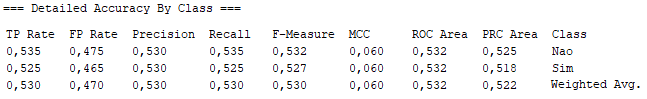
\includegraphics[scale=0.93]{Figuras/Tabela_de_acuracia_das_classes.png}
	\end{center}
    \legend{Fonte: Próprio autor.}
\end{figure}

\textcolor{red}{A Figura XX, que apresenta matriz de classificação para cada classe, indica que, na classe Nao, de 779 ocorrências, apenas 366 registros foram classificados corretamente, enquanto na classe Sim, de 795 ocorrências, apenas 374 registros foram classificados corretamente.}

\par
\begin{figure}[!htp]
	\begin{center}
    \caption{\label{fig:waveform_fig} Matriz de confusão.}
	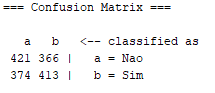
\includegraphics[scale=0.99]{Figuras/Matriz_de_classificacao.png}
	\end{center}
    \legend{Fonte: Próprio autor.}
\end{figure}

\par
\textcolor{red}{Podemos notar que a taxa de acurácia do modelo utilizado, deu como resultado aproximadamente 53\% de instancias classificadas corretamente, um valor um pouco abaixo do que esperado, que era de 70\% de precisão para ser um bom modelo. Como foi explicado durante a preparação do modelo, que foi necessário utilizar técnicas para balancear os dados com o intuito de resolver o problema de classe rara, teve como consequência, uma queda drástica da quantidade de registros, onde, de 8.571 registros caiu para 1.574 registros balanceados. Por causa desse balanceamento, foi um dos fatores que motivaram para que o modelo não possuísse registros suficiente a fim de obter uma taxa razoável  de instâncias classificadas corretamente.}

\section{Avaliando com o algoritmo Apriori}


